%This work is licensed under the Creative Commons License Attribution 4.0 International (CC-BY 4.0)
%https://creativecommons.org/licenses/by/4.0/legalcode
\documentclass[rgb]{standalone}
\usepackage{tkz-euclide}
\definecolor{myorange}{hsb}{0.0833, 1, 0.8}
\definecolor{mygreen}{hsb}{0.3333, 1, 0.8}
\definecolor{myblue}{hsb}{0.5833, 1, 0.8}
\definecolor{mymagenta}{hsb}{0.8333, 1, 0.8}
\begin{document}
	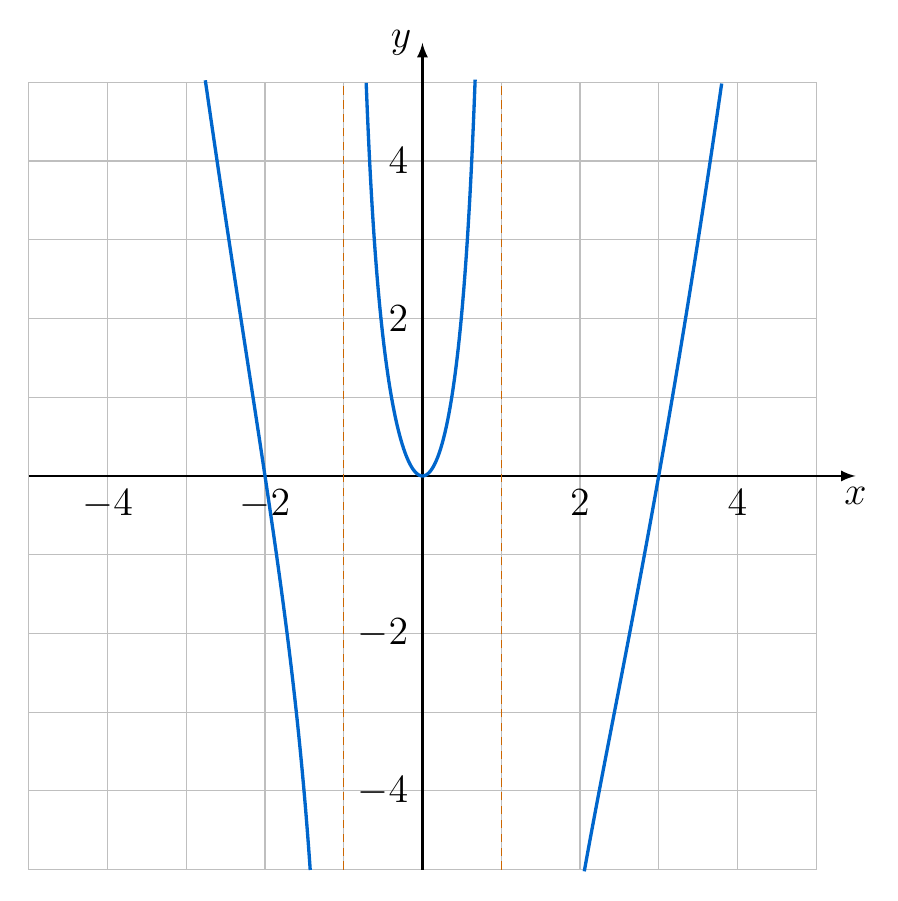
\begin{tikzpicture}[scale=1, font=\Large]
		% Coordinate system
		\tkzInit[xmin=-5,xmax=5,ymin=-5,ymax=5]
		\tkzGrid[color=lightgray]
		\tkzDrawX[thick,label=$x$]
		\tkzDrawY[thick,label=$y$]
		% Graphs
		\draw[very thick,myblue,smooth,domain={-2.758}:{-1.425},samples=100, variable=\x] plot ({\x}, {((\x)^2*(\x+2)*(\x-3))/((\x+1)*(\x-1))});
		\draw[very thick,myblue,smooth,domain={-0.715}:{0.67},samples=100, variable=\x] plot ({\x}, {((\x)^2*(\x+2)*(\x-3))/((\x+1)*(\x-1))});
        \draw[very thick,myblue,smooth,domain={2.055}:{3.8},samples=100, variable=\x] plot ({\x}, {((\x)^2*(\x+2)*(\x-3))/((\x+1)*(\x-1))});
        \draw[myorange,,densely dashed] (-1,-5) -- (-1,5);
        \draw[myorange,,densely dashed] (1,-5) -- (1,5);
		% Labels
		\node[below=0.5mm] at (-4,0){$-4$};
	    \node[below=0.5mm] at (-2,0){$-2$};
		\node[below=0.5mm] at (2,0){$2$};
		\node[below=0.5mm] at (4,0){$4$};
		\node[left=0.5mm] at (0,-4){$-4$};
		\node[left=0.5mm] at (0,-2){$-2$};
		\node[left=0.5mm] at (0,2){$2$};
		\node[left=0.5mm] at (0,4){$4$};
%		\node[right,myblue] at (-5,-3.5){$p(x)=\frac{x^4-x^3-6x^2}{x^2-1}$};
	\end{tikzpicture}	
\end{document}